\documentclass{standalone}
\usepackage{tikz}
\usetikzlibrary{patterns, positioning}


\begin{document}
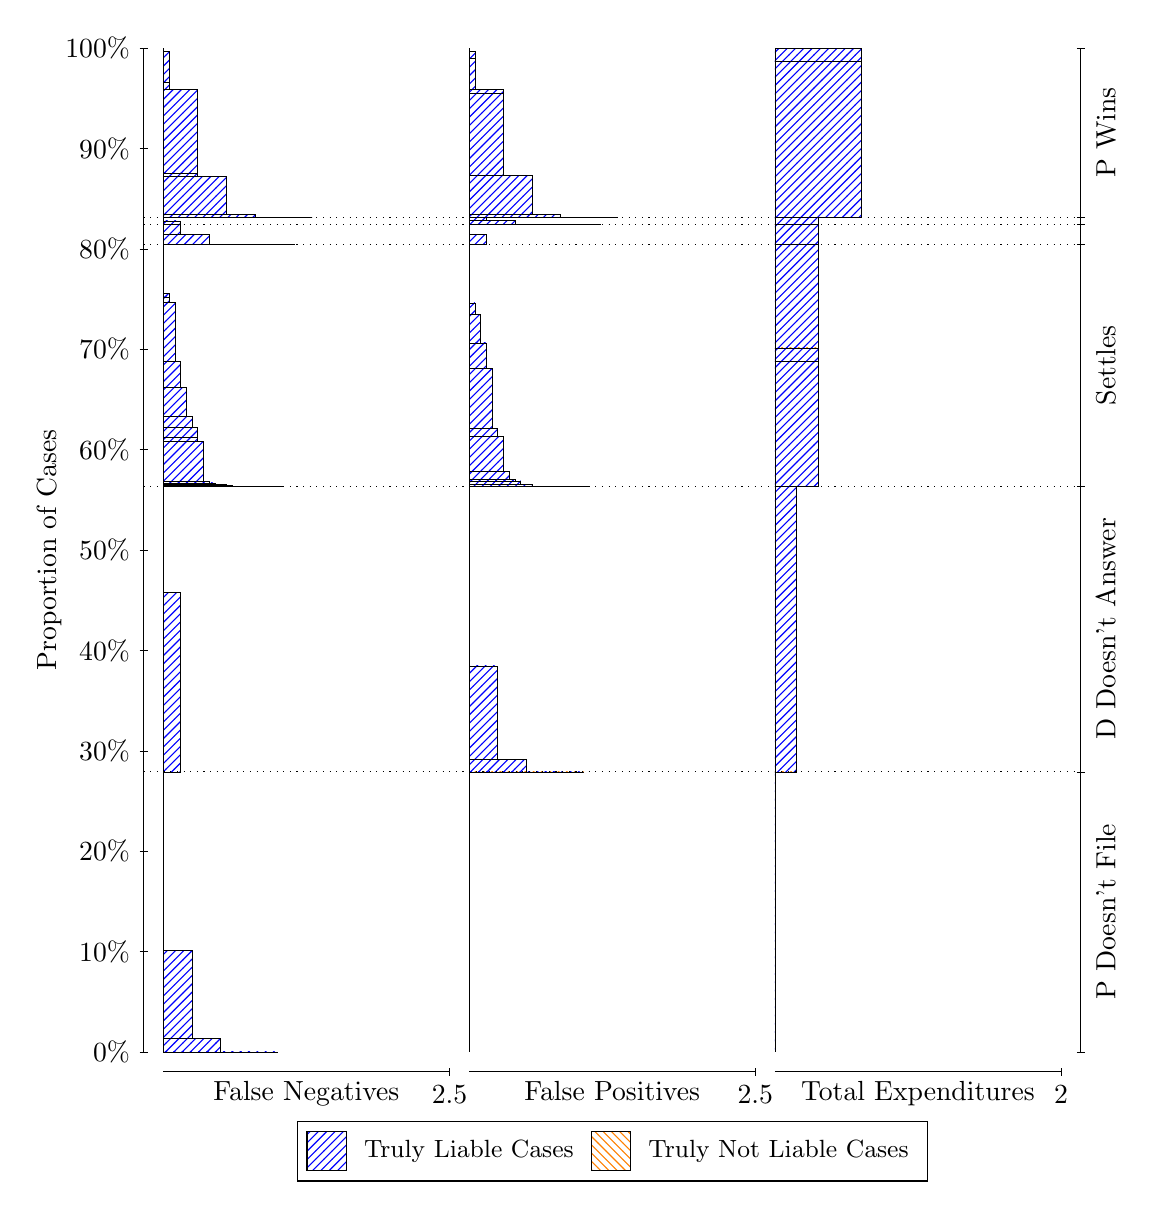
\begin{tikzpicture}
\draw[black, very thin] (1.5,1.75) -- (1.5,14.5);
\node[rotate=90, text=black, anchor=center] at (0.3, 8.125) {Proportion of Cases};
\draw[black, very thin] (1.45,1.75) -- (1.55,1.75);
\node[text=black, anchor=east] at (1.45, 1.75) {0\%};
\draw[black, very thin] (1.45,3.025) -- (1.55,3.025);
\node[text=black, anchor=east] at (1.45, 3.025) {10\%};
\draw[black, very thin] (1.45,4.3) -- (1.55,4.3);
\node[text=black, anchor=east] at (1.45, 4.3) {20\%};
\draw[black, very thin] (1.45,5.575) -- (1.55,5.575);
\node[text=black, anchor=east] at (1.45, 5.575) {30\%};
\draw[black, very thin] (1.45,6.85) -- (1.55,6.85);
\node[text=black, anchor=east] at (1.45, 6.85) {40\%};
\draw[black, very thin] (1.45,8.125) -- (1.55,8.125);
\node[text=black, anchor=east] at (1.45, 8.125) {50\%};
\draw[black, very thin] (1.45,9.4) -- (1.55,9.4);
\node[text=black, anchor=east] at (1.45, 9.4) {60\%};
\draw[black, very thin] (1.45,10.675) -- (1.55,10.675);
\node[text=black, anchor=east] at (1.45, 10.675) {70\%};
\draw[black, very thin] (1.45,11.95) -- (1.55,11.95);
\node[text=black, anchor=east] at (1.45, 11.95) {80\%};
\draw[black, very thin] (1.45,13.225) -- (1.55,13.225);
\node[text=black, anchor=east] at (1.45, 13.225) {90\%};
\draw[black, very thin] (1.45,14.5) -- (1.55,14.5);
\node[text=black, anchor=east] at (1.45, 14.5) {100\%};

\draw[black, very thin] (13.4,1.75) -- (13.4,14.5);
\draw[black, very thin] (13.35,1.75) -- (13.45,1.75);
\node[anchor=west] at (13.35, 1.75) {};
\draw[black, very thin] (13.35,5.3079) -- (13.45,5.3079);
\node[anchor=west] at (13.35, 5.3079) {};
\draw[black, very thin] (13.35,8.9359) -- (13.45,8.9359);
\node[anchor=west] at (13.35, 8.9359) {};
\draw[black, very thin] (13.35,12.008) -- (13.45,12.008);
\node[anchor=west] at (13.35, 12.008) {};
\draw[black, very thin] (13.35,12.26) -- (13.45,12.26);
\node[anchor=west] at (13.35, 12.26) {};
\draw[black, very thin] (13.35,12.351) -- (13.45,12.351);
\node[anchor=west] at (13.35, 12.351) {};
\draw[black, very thin] (13.35,14.5) -- (13.45,14.5);
\node[anchor=west] at (13.35, 14.5) {};

\draw[black, very thin, pattern color=blue, pattern=north east lines] (1.75,1.75) rectangle (3.2033,1.75);
\draw[black, very thin, pattern color=blue, pattern=north east lines] (1.75,1.75) rectangle (2.84,1.7514);
\draw[black, very thin, pattern color=blue, pattern=north east lines] (1.75,1.7514) rectangle (2.4767,1.9205);
\draw[black, very thin, pattern color=blue, pattern=north east lines] (1.75,1.9205) rectangle (2.1133,3.0419);
\draw[black, very thin, pattern color=orange, pattern=north west lines] (1.75,3.0419) rectangle (1.75,3.0419);
\draw[black, very thin, pattern color=blue, pattern=north east lines] (1.75,3.0419) rectangle (1.75,5.3079);
\draw[black, very thin, pattern color=blue, pattern=north east lines] (1.75,5.3079) rectangle (1.968,7.5912);
\draw[black, very thin, pattern color=orange, pattern=north west lines] (1.75,7.5912) rectangle (1.75,7.5912);
\draw[black, very thin, pattern color=blue, pattern=north east lines] (1.75,7.5912) rectangle (1.75,8.9359);
\draw[black, very thin, pattern color=blue, pattern=north east lines] (1.75,8.9359) rectangle (3.276,8.9359);
\draw[black, very thin, pattern color=blue, pattern=north east lines] (1.75,8.9359) rectangle (2.9853,8.9359);
\draw[black, very thin, pattern color=blue, pattern=north east lines] (1.75,8.9359) rectangle (2.9127,8.9359);
\draw[black, very thin, pattern color=blue, pattern=north east lines] (1.75,8.9359) rectangle (2.6947,8.936);
\draw[black, very thin, pattern color=blue, pattern=north east lines] (1.75,8.936) rectangle (2.622,8.9504);
\draw[black, very thin, pattern color=blue, pattern=north east lines] (1.75,8.9504) rectangle (2.5493,8.9558);
\draw[black, very thin, pattern color=blue, pattern=north east lines] (1.75,8.9558) rectangle (2.404,8.9766);
\draw[black, very thin, pattern color=blue, pattern=north east lines] (1.75,8.9766) rectangle (2.3313,9.001);
\draw[black, very thin, pattern color=blue, pattern=north east lines] (1.75,9.001) rectangle (2.2587,9.5054);
\draw[black, very thin, pattern color=blue, pattern=north east lines] (1.75,9.5054) rectangle (2.186,9.5582);
\draw[black, very thin, pattern color=blue, pattern=north east lines] (1.75,9.5582) rectangle (2.186,9.6819);
\draw[black, very thin, pattern color=blue, pattern=north east lines] (1.75,9.6819) rectangle (2.1133,9.8242);
\draw[black, very thin, pattern color=blue, pattern=north east lines] (1.75,9.8242) rectangle (2.0407,10.19);
\draw[black, very thin, pattern color=blue, pattern=north east lines] (1.75,10.19) rectangle (1.968,10.516);
\draw[black, very thin, pattern color=blue, pattern=north east lines] (1.75,10.516) rectangle (1.8953,11.273);
\draw[black, very thin, pattern color=blue, pattern=north east lines] (1.75,11.273) rectangle (1.8227,11.339);
\draw[black, very thin, pattern color=blue, pattern=north east lines] (1.75,11.339) rectangle (1.8227,11.38);
\draw[black, very thin, pattern color=orange, pattern=north west lines] (1.75,11.38) rectangle (1.75,11.38);
\draw[black, very thin, pattern color=blue, pattern=north east lines] (1.75,11.38) rectangle (1.75,12.008);
\draw[black, very thin, pattern color=blue, pattern=north east lines] (1.75,12.008) rectangle (3.4213,12.008);
\draw[black, very thin, pattern color=blue, pattern=north east lines] (1.75,12.008) rectangle (3.058,12.008);
\draw[black, very thin, pattern color=blue, pattern=north east lines] (1.75,12.008) rectangle (2.6947,12.011);
\draw[black, very thin, pattern color=blue, pattern=north east lines] (1.75,12.011) rectangle (2.3313,12.138);
\draw[black, very thin, pattern color=blue, pattern=north east lines] (1.75,12.138) rectangle (1.968,12.26);
\draw[black, very thin, pattern color=orange, pattern=north west lines] (1.75,12.26) rectangle (1.75,12.26);
\draw[black, very thin, pattern color=blue, pattern=north east lines] (1.75,12.26) rectangle (1.968,12.304);
\draw[black, very thin, pattern color=orange, pattern=north west lines] (1.75,12.304) rectangle (1.75,12.304);
\draw[black, very thin, pattern color=blue, pattern=north east lines] (1.75,12.304) rectangle (1.75,12.351);
\draw[black, very thin, pattern color=blue, pattern=north east lines] (1.75,12.351) rectangle (3.6393,12.351);
\draw[black, very thin, pattern color=blue, pattern=north east lines] (1.75,12.351) rectangle (3.276,12.351);
\draw[black, very thin, pattern color=blue, pattern=north east lines] (1.75,12.351) rectangle (2.9127,12.389);
\draw[black, very thin, pattern color=blue, pattern=north east lines] (1.75,12.389) rectangle (2.5493,12.873);
\draw[black, very thin, pattern color=blue, pattern=north east lines] (1.75,12.873) rectangle (2.186,12.913);
\draw[black, very thin, pattern color=blue, pattern=north east lines] (1.75,12.913) rectangle (2.186,13.971);
\draw[black, very thin, pattern color=blue, pattern=north east lines] (1.75,13.971) rectangle (1.8227,14.071);
\draw[black, very thin, pattern color=blue, pattern=north east lines] (1.75,14.071) rectangle (1.8227,14.462);
\draw[black, very thin, pattern color=orange, pattern=north west lines] (1.75,14.462) rectangle (1.75,14.462);
\draw[black, very thin, pattern color=blue, pattern=north east lines] (1.75,14.462) rectangle (1.75,14.5);
\draw[black, very thin, pattern color=orange, pattern=north west lines] (5.6333,1.75) rectangle (5.6333,1.75);
\draw[black, very thin, pattern color=blue, pattern=north east lines] (5.6333,1.75) rectangle (5.6333,5.3079);
\draw[black, very thin, pattern color=orange, pattern=north west lines] (5.6333,5.3079) rectangle (7.0867,5.3079);
\draw[black, very thin, pattern color=blue, pattern=north east lines] (5.6333,5.3079) rectangle (7.0867,5.3079);
\draw[black, very thin, pattern color=blue, pattern=north east lines] (5.6333,5.3079) rectangle (6.7233,5.3084);
\draw[black, very thin, pattern color=blue, pattern=north east lines] (5.6333,5.3084) rectangle (6.36,5.469);
\draw[black, very thin, pattern color=blue, pattern=north east lines] (5.6333,5.469) rectangle (5.9967,6.6527);
\draw[black, very thin, pattern color=blue, pattern=north east lines] (5.6333,6.6527) rectangle (5.6333,8.9359);
\draw[black, very thin, pattern color=orange, pattern=north west lines] (5.6333,8.9359) rectangle (7.1593,8.9359);
\draw[black, very thin, pattern color=blue, pattern=north east lines] (5.6333,8.9359) rectangle (7.1593,8.9359);
\draw[black, very thin, pattern color=orange, pattern=north west lines] (5.6333,8.9359) rectangle (6.8687,8.9359);
\draw[black, very thin, pattern color=blue, pattern=north east lines] (5.6333,8.9359) rectangle (6.8687,8.9359);
\draw[black, very thin, pattern color=blue, pattern=north east lines] (5.6333,8.9359) rectangle (6.796,8.936);
\draw[black, very thin, pattern color=orange, pattern=north west lines] (5.6333,8.936) rectangle (6.7233,8.936);
\draw[black, very thin, pattern color=blue, pattern=north east lines] (5.6333,8.936) rectangle (6.7233,8.936);
\draw[black, very thin, pattern color=orange, pattern=north west lines] (5.6333,8.936) rectangle (6.578,8.936);
\draw[black, very thin, pattern color=blue, pattern=north east lines] (5.6333,8.936) rectangle (6.578,8.936);
\draw[black, very thin, pattern color=blue, pattern=north east lines] (5.6333,8.936) rectangle (6.5053,8.9362);
\draw[black, very thin, pattern color=blue, pattern=north east lines] (5.6333,8.9362) rectangle (6.4327,8.9616);
\draw[black, very thin, pattern color=blue, pattern=north east lines] (5.6333,8.9616) rectangle (6.36,8.9622);
\draw[black, very thin, pattern color=orange, pattern=north west lines] (5.6333,8.9622) rectangle (6.2873,8.9622);
\draw[black, very thin, pattern color=blue, pattern=north east lines] (5.6333,8.9622) rectangle (6.2873,9.0024);
\draw[black, very thin, pattern color=blue, pattern=north east lines] (5.6333,9.0024) rectangle (6.2147,9.0216);
\draw[black, very thin, pattern color=blue, pattern=north east lines] (5.6333,9.0216) rectangle (6.142,9.1279);
\draw[black, very thin, pattern color=blue, pattern=north east lines] (5.6333,9.1279) rectangle (6.0693,9.5641);
\draw[black, very thin, pattern color=orange, pattern=north west lines] (5.6333,9.5641) rectangle (5.9967,9.5641);
\draw[black, very thin, pattern color=blue, pattern=north east lines] (5.6333,9.5641) rectangle (5.9967,9.671);
\draw[black, very thin, pattern color=blue, pattern=north east lines] (5.6333,9.671) rectangle (5.924,10.429);
\draw[black, very thin, pattern color=blue, pattern=north east lines] (5.6333,10.429) rectangle (5.8513,10.754);
\draw[black, very thin, pattern color=blue, pattern=north east lines] (5.6333,10.754) rectangle (5.7787,11.12);
\draw[black, very thin, pattern color=blue, pattern=north east lines] (5.6333,11.12) rectangle (5.706,11.262);
\draw[black, very thin, pattern color=blue, pattern=north east lines] (5.6333,11.262) rectangle (5.6333,12.008);
\draw[black, very thin, pattern color=orange, pattern=north west lines] (5.6333,12.008) rectangle (5.8513,12.008);
\draw[black, very thin, pattern color=blue, pattern=north east lines] (5.6333,12.008) rectangle (5.8513,12.13);
\draw[black, very thin, pattern color=blue, pattern=north east lines] (5.6333,12.13) rectangle (5.6333,12.26);
\draw[black, very thin, pattern color=orange, pattern=north west lines] (5.6333,12.26) rectangle (7.3047,12.26);
\draw[black, very thin, pattern color=blue, pattern=north east lines] (5.6333,12.26) rectangle (7.3047,12.26);
\draw[black, very thin, pattern color=blue, pattern=north east lines] (5.6333,12.26) rectangle (6.9413,12.26);
\draw[black, very thin, pattern color=blue, pattern=north east lines] (5.6333,12.26) rectangle (6.578,12.261);
\draw[black, very thin, pattern color=blue, pattern=north east lines] (5.6333,12.261) rectangle (6.2147,12.307);
\draw[black, very thin, pattern color=blue, pattern=north east lines] (5.6333,12.307) rectangle (5.8513,12.351);
\draw[black, very thin, pattern color=orange, pattern=north west lines] (5.6333,12.351) rectangle (7.5227,12.351);
\draw[black, very thin, pattern color=blue, pattern=north east lines] (5.6333,12.351) rectangle (7.5227,12.351);
\draw[black, very thin, pattern color=orange, pattern=north west lines] (5.6333,12.351) rectangle (7.1593,12.351);
\draw[black, very thin, pattern color=blue, pattern=north east lines] (5.6333,12.351) rectangle (7.1593,12.351);
\draw[black, very thin, pattern color=orange, pattern=north west lines] (5.6333,12.351) rectangle (6.796,12.351);
\draw[black, very thin, pattern color=blue, pattern=north east lines] (5.6333,12.351) rectangle (6.796,12.389);
\draw[black, very thin, pattern color=orange, pattern=north west lines] (5.6333,12.389) rectangle (6.4327,12.389);
\draw[black, very thin, pattern color=blue, pattern=north east lines] (5.6333,12.389) rectangle (6.4327,12.88);
\draw[black, very thin, pattern color=blue, pattern=north east lines] (5.6333,12.88) rectangle (6.0693,13.924);
\draw[black, very thin, pattern color=orange, pattern=north west lines] (5.6333,13.924) rectangle (6.0693,13.924);
\draw[black, very thin, pattern color=blue, pattern=north east lines] (5.6333,13.924) rectangle (6.0693,13.977);
\draw[black, very thin, pattern color=blue, pattern=north east lines] (5.6333,13.977) rectangle (5.706,14.368);
\draw[black, very thin, pattern color=blue, pattern=north east lines] (5.6333,14.368) rectangle (5.706,14.462);
\draw[black, very thin, pattern color=blue, pattern=north east lines] (5.6333,14.462) rectangle (5.6333,14.5);
\draw[black, very thin, pattern color=orange, pattern=north west lines] (9.5167,1.75) rectangle (9.5167,1.75);
\draw[black, very thin, pattern color=blue, pattern=north east lines] (9.5167,1.75) rectangle (9.5167,5.3079);
\draw[black, very thin, pattern color=orange, pattern=north west lines] (9.5167,5.3079) rectangle (9.7892,5.3079);
\draw[black, very thin, pattern color=blue, pattern=north east lines] (9.5167,5.3079) rectangle (9.7892,8.9359);
\draw[black, very thin, pattern color=orange, pattern=north west lines] (9.5167,8.9359) rectangle (10.062,8.9359);
\draw[black, very thin, pattern color=blue, pattern=north east lines] (9.5167,8.9359) rectangle (10.062,10.522);
\draw[black, very thin, pattern color=orange, pattern=north west lines] (9.5167,10.522) rectangle (10.062,10.522);
\draw[black, very thin, pattern color=blue, pattern=north east lines] (9.5167,10.522) rectangle (10.062,10.692);
\draw[black, very thin, pattern color=orange, pattern=north west lines] (9.5167,10.692) rectangle (10.062,10.692);
\draw[black, very thin, pattern color=blue, pattern=north east lines] (9.5167,10.692) rectangle (10.062,12.008);
\draw[black, very thin, pattern color=orange, pattern=north west lines] (9.5167,12.008) rectangle (10.062,12.008);
\draw[black, very thin, pattern color=blue, pattern=north east lines] (9.5167,12.008) rectangle (10.062,12.26);
\draw[black, very thin, pattern color=orange, pattern=north west lines] (9.5167,12.26) rectangle (10.062,12.26);
\draw[black, very thin, pattern color=blue, pattern=north east lines] (9.5167,12.26) rectangle (10.062,12.351);
\draw[black, very thin, pattern color=orange, pattern=north west lines] (9.5167,12.351) rectangle (10.607,12.351);
\draw[black, very thin, pattern color=blue, pattern=north east lines] (9.5167,12.351) rectangle (10.607,14.326);
\draw[black, very thin, pattern color=orange, pattern=north west lines] (9.5167,14.326) rectangle (10.607,14.326);
\draw[black, very thin, pattern color=blue, pattern=north east lines] (9.5167,14.326) rectangle (10.607,14.5);
\draw[black, dotted] (1.5,5.3079) -- (13.4,5.3079);
\draw[black, dotted] (1.5,8.9359) -- (13.4,8.9359);
\draw[black, dotted] (1.5,12.008) -- (13.4,12.008);
\draw[black, dotted] (1.5,12.26) -- (13.4,12.26);
\draw[black, dotted] (1.5,12.351) -- (13.4,12.351);
\draw[black, very thin] (1.75,1.5) -- (5.3833,1.5);
\node[text=black, anchor=north] at (3.5667, 1.5) {False Negatives};
\draw[black, very thin] (5.3833,1.45) -- (5.3833,1.55);
\node[text=black, anchor=north] at (5.3833, 1.45) {2.5};

\draw[black, very thin] (5.6333,1.5) -- (9.2667,1.5);
\node[text=black, anchor=north] at (7.45, 1.5) {False Positives};
\draw[black, very thin] (9.2667,1.45) -- (9.2667,1.55);
\node[text=black, anchor=north] at (9.2667, 1.45) {2.5};

\draw[black, very thin] (9.5167,1.5) -- (13.15,1.5);
\node[text=black, anchor=north] at (11.333, 1.5) {Total Expenditures};
\draw[black, very thin] (13.15,1.45) -- (13.15,1.55);
\node[text=black, anchor=north] at (13.15, 1.45) {2};

\node[text=black, centered, rotate=90] at (13.72, 3.529) {P Doesn't File};
\node[text=black, centered, rotate=90] at (13.72, 7.1219) {D Doesn't Answer};
\node[text=black, centered, rotate=90] at (13.72, 10.472) {Settles};


\node[text=black, centered, rotate=90] at (13.72, 13.425) {P Wins};

\draw (7.449999999999999,1.5) node[draw=none] (baseCoordinate) {};
\begin{scope}[align=center]
        \matrix[scale=0.5, draw=black, below=0.5cm of baseCoordinate, nodes={draw}, column sep=0.1cm]{
            \node[rectangle, draw, minimum width=0.5cm, minimum height=0.5cm, pattern color=blue, pattern=north east lines] {}; &
            \node[draw=none, font=\small, text=black] (B) {Truly Liable Cases}; &
            \node[rectangle, draw, minimum width=0.5cm, minimum height=0.5cm, pattern color=orange, pattern=north west lines] {}; &
            \node[draw=none, font=\small, text=black] (B) {Truly Not Liable Cases}; \\
            };
\end{scope}

\end{tikzpicture}
\end{document}